\documentclass[12pt, letter]{exam}
\usepackage[utf8]{inputenc}
\usepackage[T1]{fontenc}
\usepackage[spanish]{babel}
\usepackage{amsmath}
\usepackage{amsthm}
\usepackage{physics}
\usepackage{tikz}
\usepackage{float}
\usepackage{siunitx}
\usepackage{multicol}
\usepackage[left=2.00cm, right=2.00cm, top=2.00cm, 
     bottom=2.00cm]{geometry}
\usepackage{pdfpages}

% \renewcommand{\questionlabel}{\thequestion}
\decimalpoint

\setlength{\belowdisplayskip}{-0.5pt}

\usepackage{tasks}
\settasks{
    label=\Alph*), 
    label-align=left,
    item-indent={20pt}, 
    column-sep={4pt},
    label-width={16pt},
}

\sisetup{per-mode=symbol}
\footer{}{\thepage}{}

\begin{document}

\includepdf[pages={1}]{Caratula_Examen_Parcial_PU_Fisica_3_02.pdf}

\newpage

    \begin{questions}
        \question Resuelve la siguiente operación con notación científica, ocupa 4 dígitos decimales en el resultado.
        \begin{align*}
        \dfrac{\num{2.7d4} - \num{1.2e3}}{[(0.013)^{2}  \times \sqrt{\num{5.6d5}}]} =
        \end{align*}
        \begin{tasks}(4)
            \task \num{2.0680d5}
            \task \num{2.9068d5}
            \task \num{2.1022d5}
            \task \num{2.6817d5}
        \end{tasks}
        \question \textbf{Ejercicio de ejecución.} ¿Cuántos nanosegundos hay un año de $365$ días?
        \begin{tasks}(4)
            \task \SI{3.1536d12}{\nano\second}
            \task \SI{3.1536d14}{\nano\second}
            \task \SI{3.1536d15}{\nano\second}
            \task \SI{3.1536d16}{\nano\second}
        \end{tasks}
        \question \textbf{Ejercicio de ejecución.} Si la velocidad del tren bala es de \SI{603}{\kilo\meter\per\hour}. ¿Qué distancia ha recorrido en \SI{1}{\minute}?
        \begin{tasks}(4)
            \task \SI{11050}{\meter}
            \task \SI{10015}{\meter}
            \task \SI{10050}{\meter}
            \task \SI{10055}{\meter}
        \end{tasks}
        \question Es la unidad de intensidad de corriente eléctrica:
        \begin{tasks}(4)
            \task Candela
            \task Ampere
            \task Kelvin
            \task Poise
        \end{tasks}
        \question En la siguiente figura se muestran dos rutas para llegar al Estadio Azteca saliendo del Museo Nacional de Antropología. Para la ruta A se cubre una distancia de \SI{21.1}{\kilo\meter}, mientras que para la ruta B, se cubre una distancia de \SI{19.5}{\kilo\meter}.
    \begin{figure}[H]
        \centering
        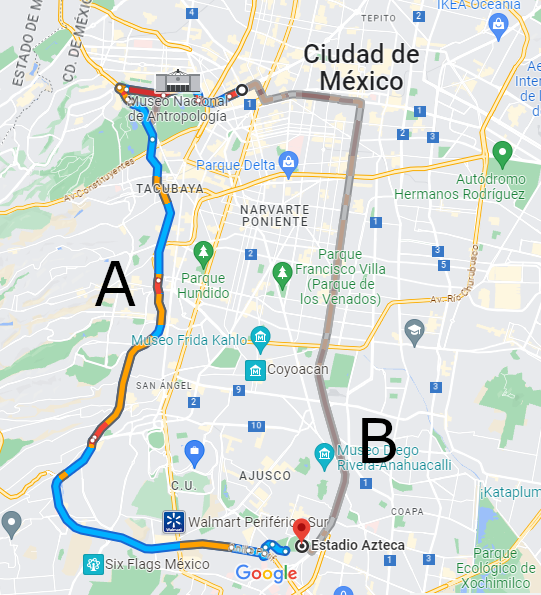
\includegraphics[scale=0.5]{Imagenes/Trayectoria_04.png}
    \end{figure}
    El desplazamiento del Museo Nacional de Antropología al Estadio Azteca con respecto a las rutas:
    \begin{tasks}(4)
        \task Es mayor en A.
        \task Es mayor en B.
        \task Es el mismo.
        \task Es $A + B$
    \end{tasks}
    \question Se tienen $4$ objetos con los siguientes datos: \\
    Objeto 1: $d = \SI{20}{\meter}, \, t = \SI{5}{\second}$ \\
    Objeto 2: $d = \SI{60}{\meter}, \, t = \SI{6}{\second}$ \\
    Objeto 3: $d = \SI{24}{\meter}, \, t = \SI{3}{\second}$ \\
    Objeto 4: $d = \SI{40}{\meter}, \, t = \SI{2}{\second}$ \\[0.3em]
    ¿Cuál de los objetos se desplazó con mayor velocidad? 
    \begin{tasks}(4)
        \task Objeto 1
        \task Objeto 2
        \task Objeto 3
        \task Objeto 4        
    \end{tasks}
    Para las preguntas \textbf{\ref{grafica_01}}, \textbf{\ref{grafica_02}}, \textbf{\ref{grafica_03}} y \textbf{\ref{grafica_04}}, considera que con los datos de la magnitud del desplazamiento de un móvil en función del tiempo, se obtuvo la siguiente gráfica:
    \begin{figure}[H]
        \centering
        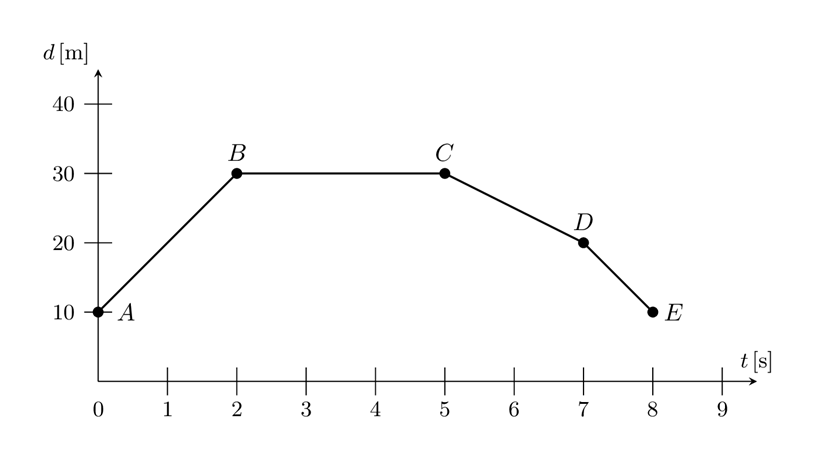
\includegraphics[scale=1.5]{Imagenes/Examen_Grafica_01.png}
    \end{figure}
    \question \label{grafica_01} ¿Qué posición tenía el móvil a los cuatro segundos posteriores al inicio de su movimiento?
    \begin{tasks}(4)
        \task \SI{0}{\meter}
        \task \SI{10}{\meter}
        \task \SI{20}{\meter}
        \task \SI{30}{\meter}
    \end{tasks}
    \question \label{grafica_02} ¿Cuál es la magnitud de la velocidad del móvil en el intervalo D - E?
    \begin{tasks}(4)
        \task \SI{0}{\meter\per\second}
        \task \SI{-5}{\meter\per\second}
        \task \SI{-10}{\meter\per\second}
        \task \SI{-20}{\meter\per\second}
    \end{tasks}
    \question \label{grafica_03} ¿Qué magnitud tiene la velocidad del móvil en el intervalo A -B?
    \begin{tasks}(4)
        \task \SI{0}{\meter\per\second}
        \task \SI{50}{\meter\per\second}
        \task \SI{10}{\meter\per\second}
        \task \SI{15}{\meter\per\second}
    \end{tasks}
    \question \label{grafica_04} ¿Cuál fue la posición final del móvil?
    \begin{tasks}(4)
        \task \SI{0}{\meter}
        \task \SI{10}{\meter}
        \task \SI{20}{\meter}
        \task \SI{30}{\meter}
    \end{tasks}
    \question \textbf{Ejercicio de ejecución.}  Una avioneta parte del reposo y alcanza una rapidez de \SI{95}{\kilo\meter\per\hour} en \SI{7}{\second} para su despegue. ¿Cuál fue la magnitud de su aceleración?
    \begin{tasks}(4)
        \task \SI{10.53}{\meter\per\square\second}
        \task \SI{13.57}{\meter\per\square\second}
        \task \SI{15.83}{\meter\per\square\second}
        \task \SI{20.10}{\meter\per\square\second}
    \end{tasks}
    \question Considera la siguiente figura ¿cuál es valor de la aceleración en el intervalo B - C?
    \begin{figure}[H]
        \centering
        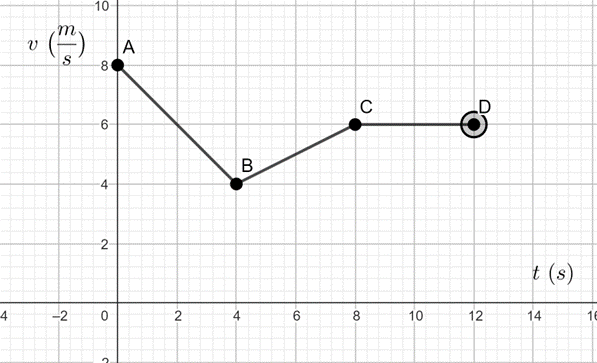
\includegraphics[scale=1.5]{Imagenes/Examen_Grafica_02.png}
    \end{figure}
    \begin{tasks}(4)
        \task \SI{0}{\meter\per\square\second}
        \task \SI{1}{\meter\per\square\second}
        \task \SI{-1}{\meter\per\square\second}
        \task \SI{-2}{\meter\per\square\second}
    \end{tasks}
    \question \textbf{Problema de ejecución:} Un auto deportivo acelera desde el reposo hasta alcanzar \SI{100}{\kilo\meter\per\hour} en \SI{4.5}{\second}. ¿Cuál es su aceleración?
    \begin{tasks}(4)
        \task \SI{5.10}{\meter\per\square\second}
        \task \SI{6.17}{\meter\per\square\second}
        \task \SI{11.11}{\meter\per\square\second}
        \task \SI{27.77}{\meter\per\square\second}
    \end{tasks}
    \question De acuerdo al Sistema Internacional de Unidades ¿cuántas son las magnitudes fundamentales?
     \begin{tasks}(4)
         \task $11$
         \task $7$
         \task $8$
         \task $10$
     \end{tasks}
     \question Si un objeto aumenta su aceleración, en la gráfica de velocidad contra tiempo la pendiente de la recta que describe el movimiento del objeto es:
    \begin{tasks}(4)
        \task Positiva
        \task Negativa
        \task Cero
        \task Concomitante        
    \end{tasks}
    \question \textbf{(5 puntos)} A continuación se te presenta la definición de 5 conceptos, la palabra faltante está en la parte inferior, relaciona cada definición con la palabra.
    \begin{parts}
        \part \rule{2cm}{0.3mm} es comparar una magnitud con un patrón.
        \part Cuando hablamos de la razón de cambio del desplazamiento con respecto al tiempo, hablamos de  \rule{2cm}{0.3mm}.
        \part \rule{2cm}{0.3mm} es la distancia recorrida por unidad de tiempo.
        \part \rule{1.5cm}{0.3mm} es la razón de cambio de la velocidad con respecto al tiempo.
        \part \rule{2cm}{0.3mm} es el cambio de posición de un objeto dentro de un espacio determinado.
    \end{parts}
    
    \begin{center}
    I) Velocidad, \hspace{0.2cm} II) Aceleración, \hspace{0.2cm} III) Sistema de referencia, \hspace{0.2cm} IV) Magnitud, \\[0.5em] V) Movimiento, \hspace{0.2cm} VI) Medir, \hspace{0.2cm} VII) Rapidez
    \end{center}
    {
    \renewcommand{\thepartno}{\Alph{partno}}
    \renewcommand{\partlabel}{\thepartno)}
    \begin{parts}
        \part a) - VI), b) - II), c) - VII), d) - II) e) - V)
        \part a) - VI), b) - VII), c) - IV), d) - V) e) - VI)
        \part a) - VII), b) - VI), c) - I), d) - V) e) - III)
        \part a) - III), b) - IV), c) - VII), d) - II) e) - I)
    \end{parts}}

    \end{questions}

\newpage
\textbf{\huge{Formulario.}}
\begin{table}[H]
    \centering
    \setlength{\tabcolsep}{40pt}
    \renewcommand{\arraystretch}{2.5}
    \begin{tabular}{c  c}
            $v = \dfrac{d}{t}$ & $v = \dfrac{x_{f} - x_{i}}{t_{f} - t_{i}}$ \\
            $a = \dfrac{v_{f} - v_{i}}{t}$ & $v_{f} = v_{i} + a \, t$ \\
            $v_{f}^{2} = v_{i}^{2} + 2 \, a \, \left(x_{f} - x_{i} \right)$ & $x_{f} = x_{i} + v_{i} + \dfrac{1}{2} \, a \, t^{2}$ \\
            $x_{f} = x_{i} + \dfrac{1}{2} \, \left(v_{i} + v_{f} \right) \, t$ & $g = \SI{9.81}{\meter\per\square\second}$ \\
            $h =\dfrac{1}{2} \,g \, t^{2}$ & \\
\end{tabular}
\end{table}
\end{document}